\section{Speech and Person Recognition}
The robot has to identify unknown people and answer questions about them and the environment.

\subsection{Focus}
This test focuses on human detection, sound localization, speech recognition, and robot interaction with unknown people.

\subsection{Setup}
\begin{enumerate}
    \item \textbf{Location:} One room of the arena is used for this test\footnote{This test may also be held outside the arena}.
    \item \textbf{Crowd:} There is a crowd of 5 to 10 people in the designated room. People may be standing, sitting, lying, and in any pose.
    \item \textbf{Doors:} All doors of the apartment are open, except for the entry door.
\end{enumerate}

\subsection{Task}
\begin{enumerate}
    \item \textbf{Start:} The robot starts at a designated starting position and announces it wants \textit{to play riddles}.

    \item \textbf{Waiting and turn:} After stating that it wants \textit{to play a riddle game}, the robot waits for 10 seconds while a crowd is merged on it's back. When the time elapses, the robot must turn around (about $180\degree$) and find the crowd.

    \item \textbf{Requesting an operator:} After turning around, the robot must state the size of the crowd (including male and female count\footnotemark) and request for an operator (e.g.~\textit{who want to play riddles with me?}). The crowd will move and surround the robot, letting the operator to stand in front of the robot.
    \footnotetext{It is possible to state the number of people whose gender couldn't be determined by the robot, therefore stating correctly the size of the crowd and, possibly, one of the gender groups.}

    \item \textbf{The riddle game:} Standing in front of the robot, the operator will ask 5 questions.\\
    The robot must answer the question without asking confirmation. Questions will only be asked only once; no repetitions are allowed.

    \newcounter{enumTempSPR}
    \setcounter{enumTempSPR}{\theenumi}
    \item {[DSPL only]} \textbf{Blind man's bluff game: Crowd line-up.} The crowd will reposition, lining up in front of the robot. A random person from the crowd standing in front of the robot will ask a question. The robot may
    \begin{itemize}
        \item Turn towards the person who asked the question and answer the question
        \item Directly answer the question without turning
        \item Turn towards the person and ask them to repeat the question
    \end{itemize}
    This process is repeated with 10 (possibly) different people.
    The game will end when the 10th question has been made, following a similar distribution of questions as in the riddle game. The robot must answer the question without asking confirmation. Questions may be repeated once.

    \setcounter{enumi}{\theenumTempSPR}
    \item {[OPL \& SSPL]} \textbf{Blind man's bluff game: Circling Crowd.} The crowd will reposition, making a circle around the robot. A random person from the crowd surrounding the robot will ask a question. The robot may
    \begin{itemize}
        \item Turn towards the person who asked the question and answer the question
        \item Directly answer the question without turning
        \item Turn towards the person and ask them to repeat the question
    \end{itemize}
    This process is repeated with 5 (possibly) different people.
    The game will end when the 5th question has been made, following the same distribution of questions as in the riddle game. The robot must answer the question without asking confirmation. Questions may be repeated once.

    \item \textbf{Leave} The robot must leave the arena/test area after all questions have been asked or when instructed to do so.
\end{enumerate}

\subsection{Additional rules and remarks}

\begin{enumerate}
    \item \textbf{Bypassing ASR:} Bypassing Automated Speech Recognition via the CONTINUE rule (see~\refsec{rule:asrcontinue}) is not allowed during this test.
    \item \textbf{Asked questions:} The distribution of questions to be randomly asked is a follows:
    \begin{itemize}
        \item One is a predefined question
        \item Between one and two are about the arena and its status
        \item Between one and two are about the crowd
        \item Between one and two are about the list of official objects
    \end{itemize}
    Question examples see Appendix~\refsec{chap:robogame-appendix}. Questions are generated by the generator which is made publicly available at https://github.com/kyordhel/GPSRCmdGen.
    \item \textbf{Distance to the robot:} The distance between each person and the robot must be between 0.75 and 1.0 meters away from the robot position (See Figure~\ref{fig:asrsetup}). In the \textit{riddle game} the operator shall be between -60$^{\circ}$ and 60$^{\circ}$ from the robot's center (front range).
    \item \textbf{Precise turning:} When the robot finishes turning toward an operator, it must be clear that the robot is facing the person who made the question.
    \item \textbf{Question repetition:} In the \textit{blind man's bluff game}, if the robot asks for repetition, it should be done clear and loud, and after the robot has ended turning.
    \item \textbf{Question timeout:} If the robot does not answer within 10 seconds, the question is considered as \textit{missed}, and referee will proceed with the next one.
    \item \textbf{Standing still operators} Operators are not allowed to move to or turn towards the robot or shout to the robot.
    \item \textbf{Water-clear answers:} If the referee is unable to hear or understand the robot's answer, the question is considered as \textit{incorrect}. Single-word and short answers should be avoided
\end{enumerate}

\begin{figure}[!h]
	\centering
	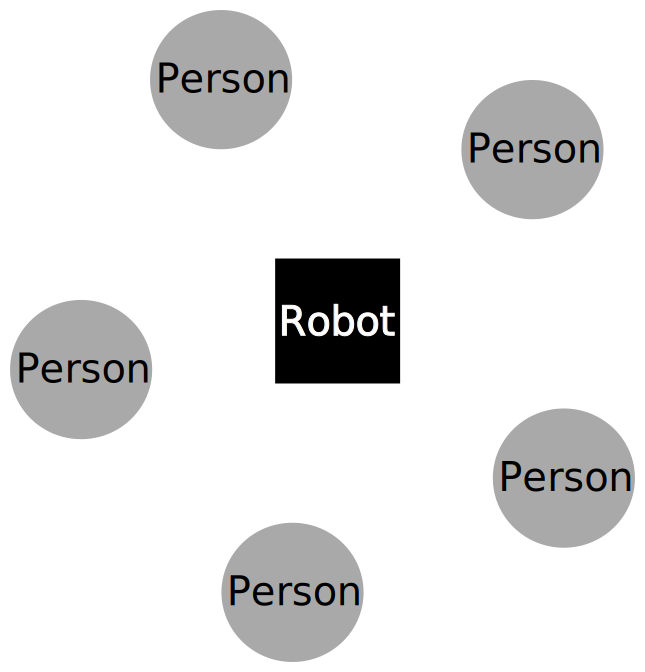
\includegraphics[width=0.5\columnwidth]{images/asrsetup.pdf}
	\caption{Speech recognition test: person setup around the robot for 2nd part.}
	\label{fig:asrsetup}
\end{figure}

% \subsection{Data recording}
% Please record the following data (See~\refsec{rule:datarecording}):
% \begin{itemize}
%     \item Audio
%     \item Commands
%     \item Images
% \end{itemize}

\subsection{Referee instructions}

The referee needs to
\begin{itemize}
    \item avoid shouting to the robot
    \item avoid getting closer to the robot (or even move)
    \item speak to the robot loud and clear with plain standard English
    \item avoid repeating questions for the same robot
    \item distribute the questions among the volunteers
\end{itemize}

\subsection{OC instructions}

\textbf{1 day before the test}
\begin{itemize}
    \item Provide the set of predefined questions
\end{itemize}

\textbf{2 hours before the test}
\begin{itemize}
    \item Announce the placement of the robots
    \item choose the volunteers for the second part of the test, and clearly explain the procedure to them.
    \item When the test is held outside the arena, announce the (way)point through which the robot shall leave
\end{itemize}

\subsection {Audio Data Recollection}
Teams are encouraged to submit to the TC the audio data recorded during the test, specially that which was captured during speech recoginition. If so, teams are urged to provide it with annotation of what the user said and what was recognized. Audio files are expected to be mono, one per microphone (in the case array recordings), of a sample rate equal to or higher than 16 kHz, and with a sample size of at least 16 bits. Depending on the quality of the recordings and their annothations, an official certificate that formalizes these efforts may be provided to submitting teams.

\newpage
\subsection{Score sheet}
The maximum time for this test is 5 minutes.

\begin{scorelist}

	\scoreheading{Crowd} % Max 15 points
	\scoreitem{ 5}{State crowd's size}
	\scoreitem{10}{State crowd's male/female count}

	\scoreheading{Riddle game} % Max 55 points
	\scoreitem[ 5]{5}{Understanding question}
	\scoreitem[ 5]{5}{Correctly answered a question}
	\scoreitem{ 5}{Answering all 5 riddle game question}

\ifDSPL{
	\scoreheading{[DSPL only] Blind man's bluff game} % Max 130
	\scoreitem[10]{ 5}{Understanding question on the first attempt}   % 50
	\scoreitem[10]{ 2}{Understanding question on the second attempt}  % -- (20)
	\scoreitem[10]{ 2}{Correctly answered a question}                 % 20
	\scoreitem[10]{ 5}{Turned towards person asking the question}     % 50
	\scoreitem{10}{Answering all 10 blind man's bluff questions}      % 10
}

\ifNotDSPL{
	\scoreheading{[OPL \& SSPL] Blind man's bluff game} % Max 130
	\scoreitem[ 5]{10}{Understanding question on the first attempt}   % 50
	\scoreitem[ 5]{ 5}{Understanding question on the second attempt}  % -- (25)
	\scoreitem[ 5]{ 5}{Correctly answered a question}                 % 25
	\scoreitem[ 5]{10}{Turned towards person asking the question}     % 50
	\scoreitem{ 5}{Answering all 5 blind man's bluff questions}       %  5	
}

	\setTotalScore{200}	
\end{scorelist}

\ifEvaluationSheet{
\textbf{Crowd setup ground truth}
\begin{figure}[!htb]
	\centering
	\begin{minipage}{.3\textwidth}
		\begin{center}
			\begin{tabular}{|l||l|l|l|l|}
				\hline
				Name & 
				\parbox[t]{2mm}{\rotatebox[origin=c]{90}{Stand}} & \parbox[t]{2mm}{\rotatebox[origin=c]{90}{Sit}} & \parbox[t]{2mm}{\rotatebox[origin=c]{90}{Lay}} & \parbox[t]{2mm}{\rotatebox[origin=c]{90}{Arm pose}}\\\hline
				× & × & × & × & ×\\\hline
				× & × & × & × & ×\\\hline
				× & × & × & × & ×\\\hline
				× & × & × & × & ×\\\hline
				× & × & × & × & ×\\\hline
				× & × & × & × & ×\\\hline
			\end{tabular}
		\end{center}
	\end{minipage}
	\begin{minipage}{.3\textwidth}
		\begin{center}
			\begin{tabular}{|l||l|l|l|l|}
				\hline
				Name & 
				\parbox[t]{2mm}{\rotatebox[origin=c]{90}{Stand}} & \parbox[t]{2mm}{\rotatebox[origin=c]{90}{Sit}} & \parbox[t]{2mm}{\rotatebox[origin=c]{90}{Lay}} & \parbox[t]{2mm}{\rotatebox[origin=c]{90}{Arm pose}}\\\hline
				× & × & × & × & ×\\\hline
				× & × & × & × & ×\\\hline
				× & × & × & × & ×\\\hline
				× & × & × & × & ×\\\hline
				× & × & × & × & ×\\\hline
				× & × & × & × & ×\\\hline
			\end{tabular}
		\end{center}
	\end{minipage}
	\begin{minipage}{.3\textwidth}
		\begin{center}
			\begin{tabular}{|l||l|l|l|l|}
				\hline
				Name & 
				\parbox[t]{2mm}{\rotatebox[origin=c]{90}{Stand}} & \parbox[t]{2mm}{\rotatebox[origin=c]{90}{Sit}} & \parbox[t]{2mm}{\rotatebox[origin=c]{90}{Lay}} & \parbox[t]{2mm}{\rotatebox[origin=c]{90}{Arm pose}}\\\hline
				× & × & × & × & ×\\\hline
				× & × & × & × & ×\\\hline
				× & × & × & × & ×\\\hline
				× & × & × & × & ×\\\hline
				× & × & × & × & ×\\\hline
				× & × & × & × & ×\\\hline
			\end{tabular}
		\end{center}
	\end{minipage}
\end{figure}
}{}
% Local Variables:
% TeX-master: "Rulebook"
% End:


% Local Variables:
% TeX-master: "Rulebook"
% End:
